
\subsection{Программная реализация серверной части конструктора}

Далее идёт обоснование выбора инструментов для реализации серверной части
конструктора и описание
разработанных программных интерфейсов модулей серверной части, а также её сервисов.



\subsubsection{Выбор инструментов разработки}

В браузере доступны следующие инструменты для создания веб-приложения:
\begin{itemize}
	\item HTML;
	\item CSS;
	\item JavaScript.
\end{itemize}

HTML (HyperText Markup Language — «язык гипертекстовой разметки»)
— самый базовый строительный блок Веба. Он определяет содержание и
структуру веб-контента.

Cascading Style Sheets (CSS) — это язык иерархических правил,
используемый для представления внешнего вида документа, написанного на
HTML. CSS описывает, каким образом элемент должен отображаться на
экране, на бумаге, голосом или с использованием других медиа средств.

JavaScript — это легковесный, интерпретируемый или JIT-
компилируемый, объектно-ориентированный язык с функциями первого
класса. Наиболее широкое применение находит как язык сценариев веб-
страниц. JavaScript это прототипно-ориентированный, мультипарадигменный
язык с динамической типизацией, который поддерживает объектно-
ориентированный, императивный и декларативный (например,
функциональное программирование) стили программирования.

Основной недостаток JavaScript – это динамическая типизация, при
которой переменная связывается с типом в момент присваивания значения, а
не в момент объявления переменной. Это особенность JS приводит к
достаточно долгой отладке кода при возникновении ошибки.

Для решения этой проблемы был выбран язык TypeScript –
компилируемый язык с возможностью явного статического назначения типов.
Статическая типизация устраняет основной недостаток JS, а компиляция
позволяет выявить некоторые ошибки до запуска приложения. Также он
совместим с JS.

Среди инструментов, облегчающих разработку клиентских приложений
в браузере, имеются:

\begin{itemize}
	\item Vue - JavaScript-фреймворк с открытым исходным кодом для
	      создания пользовательских интерфейсов. Легко интегрируется в проекты с
	      использованием других JavaScript-библиотек. Может функционировать как
	      веб-фреймворк для разработки одностраничных приложений в реактивном
	      стиле.
	\item Angular - открытая и свободная платформа для разработки веб-
	      приложений, написанная на языке TypeScript, разрабатываемая командой из
	      компании Google, а также сообществом разработчиков из различных
	      компаний.
	\item React - JavaScript-библиотека с открытым исходным кодом для
	      разработки пользовательских интерфейсов. React разрабатывается и
	      поддерживается Facebook, Instagram и сообществом отдельных разработчиков
	      и корпораций. React может использоваться для разработки одностраничных и
	      мобильных приложений. Его цель — предоставить высокую скорость
	      разработки, простоту и масштабируемость.
	\item SolidJS – это легковесная JavaScript библиотека для создания
	      пользовательских интерфейсов. SolidJS вдохновлен библиотекой React, но
	      нацелен на предоставление более простой и эффективной модели
	      программирования.
\end{itemize}

В качестве сравнения данных библиотек и фреймворков выделим
следующие критерии:
\begin{itemize}
	\item поддержка реактивности;
	\item сложность изучения;
	\item производительность;
	\item потребление памяти.
\end{itemize}

Под реактивностью понимается обновления отображения при
изменении привязанных данных.

Angular является фреймворком для создания крупных браузерных
решений. Он имеет довольно много возможностей и из-за этого имеет
довольно большой размер и сложен для обучения.

Vue является фреймворком для создания реактивных приложений.
Имеет много оптимизаций в своей основе: кэширование вычисляемых
свойств, умная перерисовка – перерисовываются только нужные узлы, что
позволяет работать приложению довольно быстро. Также легок в обучении и
не требует много памяти.

React является библиотекой для создания реактивных приложения.
Имеет немного низкую производительность, чем Vue, но обладает высокой
скоростью обучения и также предрасположен к низкому потреблению памяти.

SolidJS также является библиотекой для создания реактивных
приложений. Реактивность реализуется без использования виртуального
DOM, что увеличивает производительность библиотеки и уменьшает
потребление памяти.

Сравнение фреймворков и библиотек по критериям представлено в
таблице~\ref{t:comp-client-lib}.


\begin{table}[ht]
	\Large
	\begin{threeparttable}
		\caption{Сравнение фреймворков и библиотек JavaScript}
		\label{t:comp-client-lib}
		\centering
		\begin{tabularx}{\textwidth}
			{|>{}X
			|>{\centering\arraybackslash}X
			|>{\centering\arraybackslash}X
			|>{\centering\arraybackslash}X
			|>{\centering\arraybackslash}X|}
			\hline
			        &
			Vue.js  &
			React   &
			Angular &
			SolidJS                                         \\
			\hline
			Поддержка
			реактивности
			        & есть    & есть    & есть    & есть    \\
			\hline
			Сложность изучения
			        & низкая  & низкая  & высокая & низкая  \\
			\hline
			Про\-из\-во\-ди\-тель\-ность
			        & средняя & средняя & средняя & высокая \\
			\hline
			Потребление памяти
			        & низкое  & низкое  & высокое & низкое  \\
			\hline
		\end{tabularx}
	\end{threeparttable}
	\vspace{\bottompaddingoftable}
\end{table}



Исходя из таблицы можно сделать вывод, что SolidJS является самым
оптимальным выбором для разработки клиентской части для конструктора
Telegram-ботов.


\subsubsection{Создание базы данных}

Для хранения данных приложений была создана база данных
представляющая собой следующий набор сущностей:

пользователь конструктора;
\begin{itemize}
	\item пользователь бота;
	\item бот;
	\item группа компонентов;
	\item компонент.
\end{itemize}

Пользователь хранит логин и пароль для возможности аутентификации
его в системе.

Бот содержит такую информацию, как имя и принадлежность какому-
либо пользователю путем указания его идентификатора.

Пользователь бота содержит информацию, которая старается подробно
его описать. Сюда входят такие поля, как идентификатор телеграмма, имя,
фамилия, ник. Также для хранения текущей сессии пользователя бота
содержаться поля идентификатора компонента и контекста.

Группа компонентов содержит поля имени группы, а также поле
указания принадлежности к определенному боту. Группы позволяют
потенциально расширить возможность конструктора, введя туда компонент,
который будет отвечать за определение и вызов функций – набор
компонентов.

Компонент содержит поля типа, пути, данных, выходов,
идентификатора следующего компонента и позиции на области редактора.

ER-диаграмма представлена на рисунке~\ref{f:erd}.

\begin{figure}[ht]
	\centering
	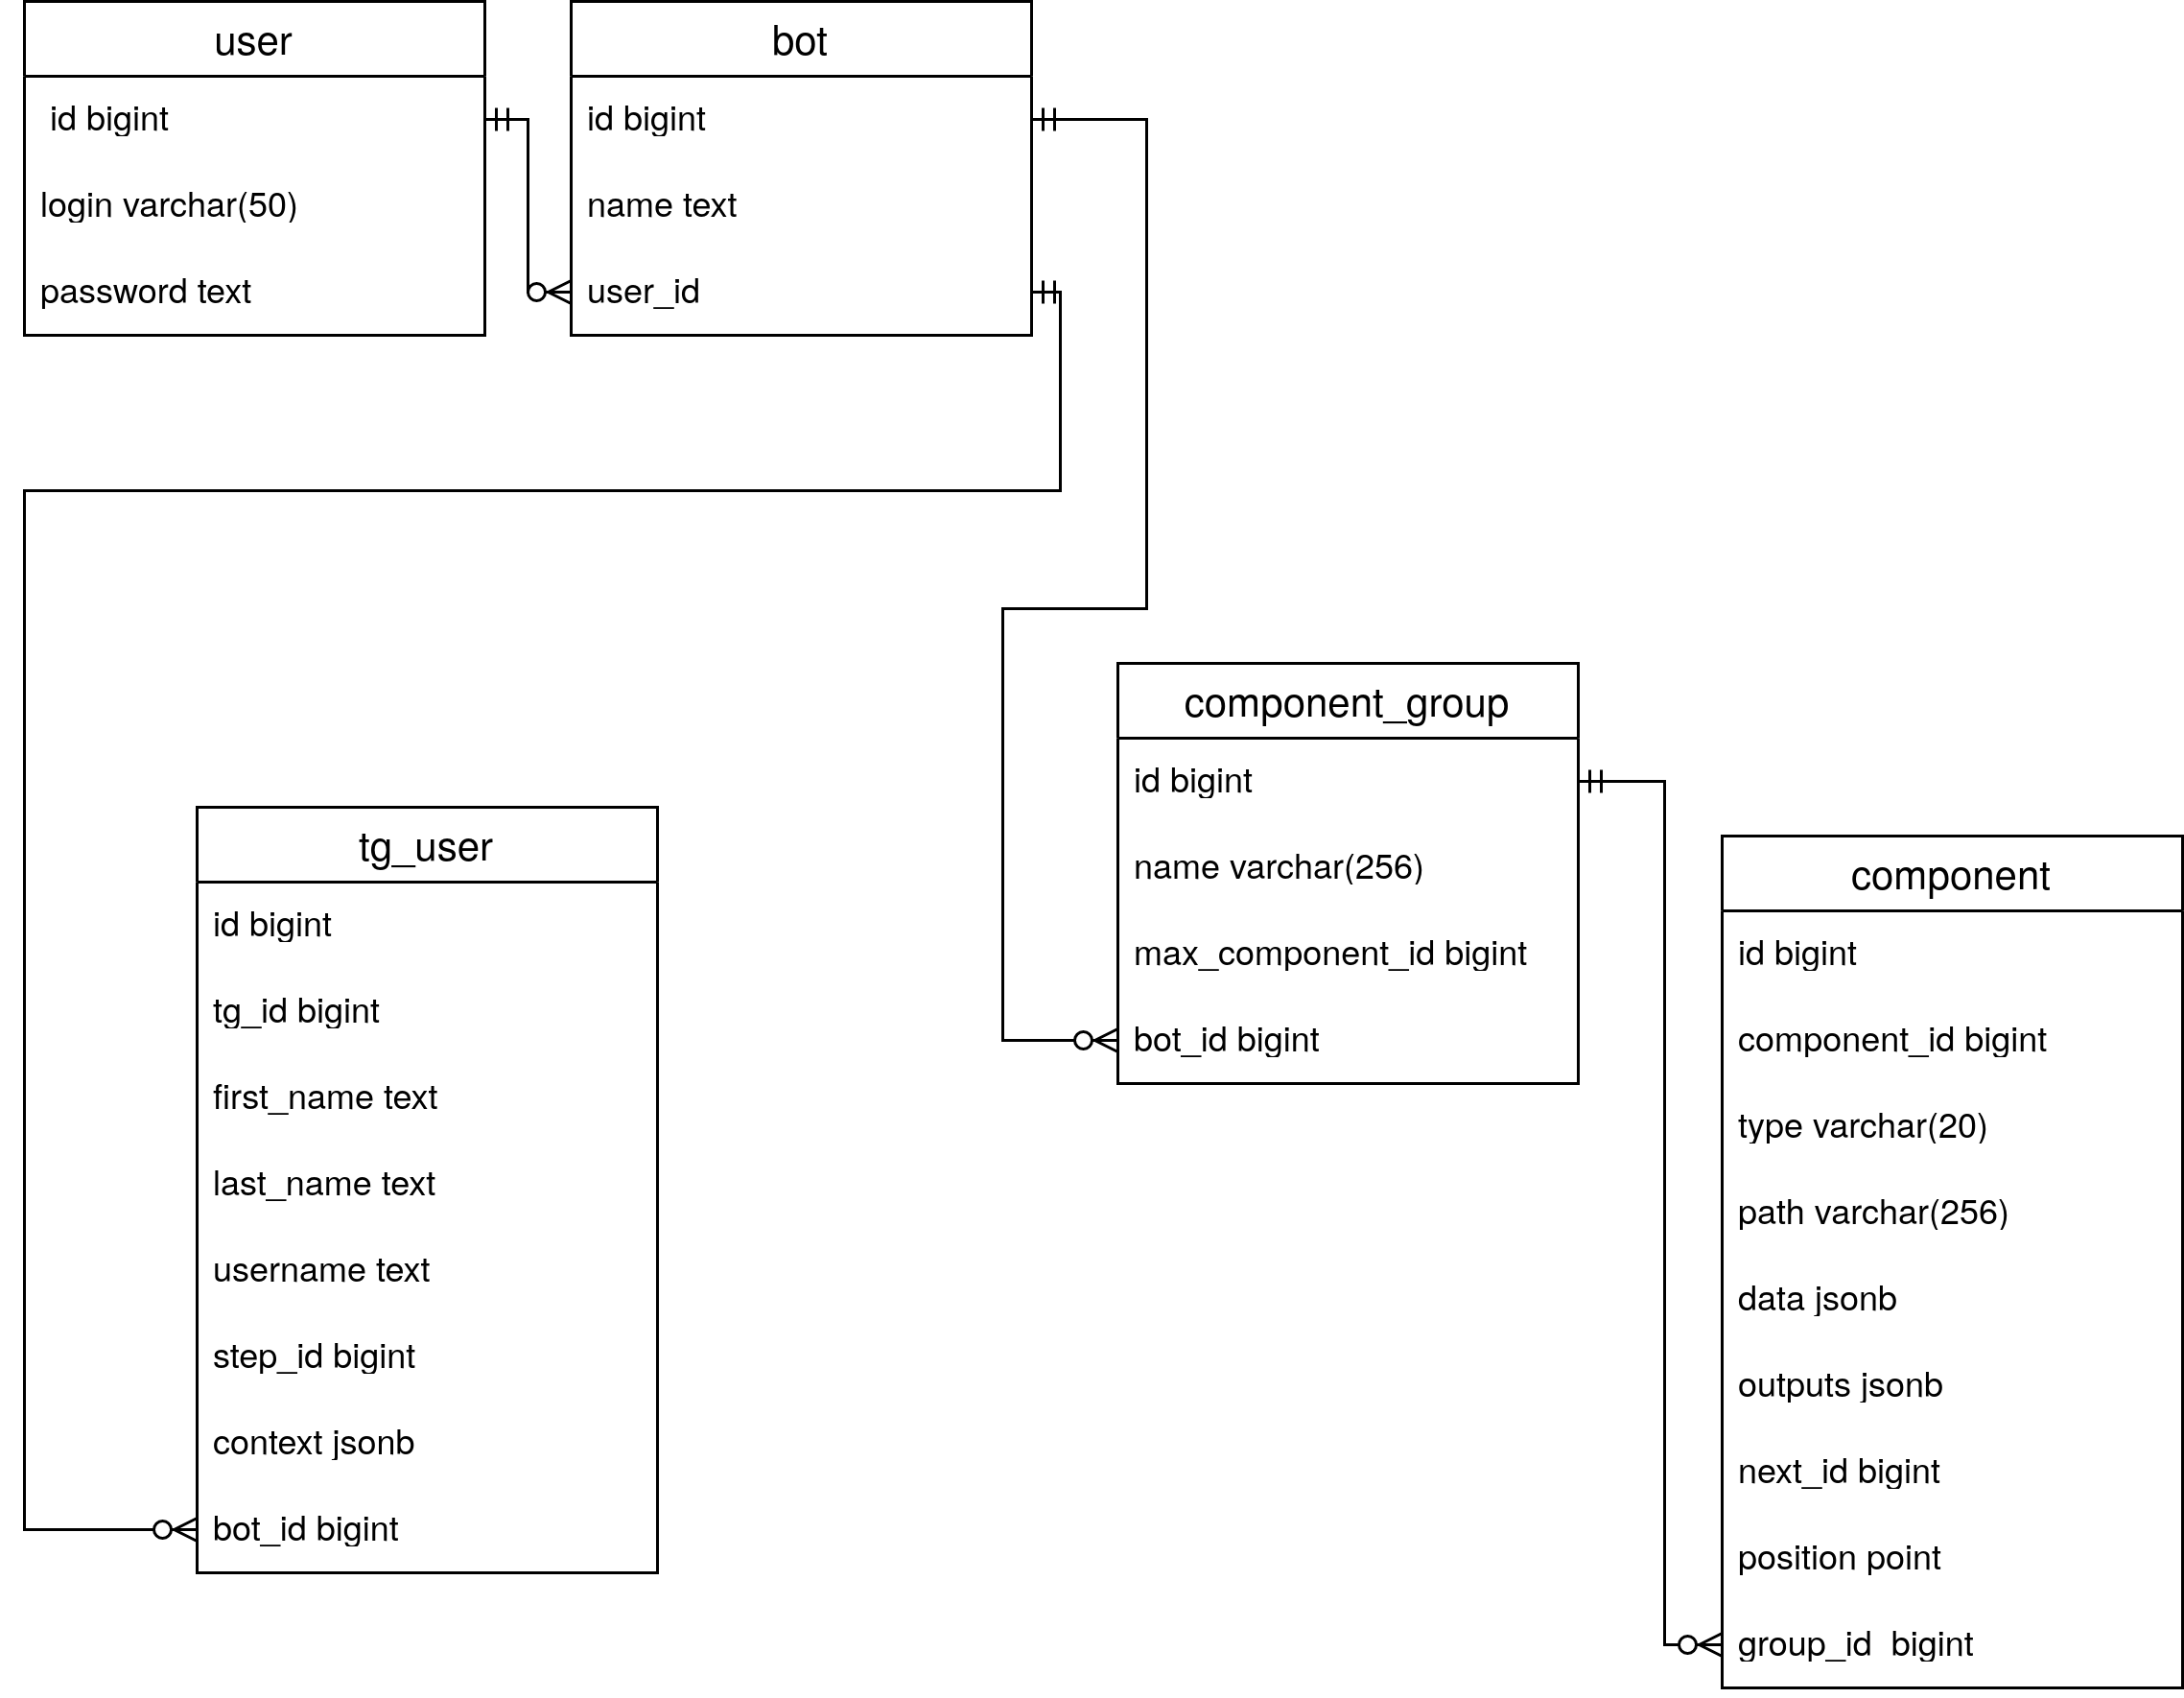
\includegraphics[width=0.95\textwidth]{db}
	\caption{Общая структура конструктора}
	\label{f:erd}
\end{figure}



\subsubsection{Реализация модуля пользователей}

Модуль пользователей предоставляет интерфейс и его реализацию для
авторизации пользователей в системе.

Интерфейс представлен на рисунке~\ref{f:auth-interface}.


\begin{figure}[ht]
	\centering
	\vspace{\toppaddingoffigure}
	\begin{lstlisting}[
        language=Go,
        xleftmargin=.1\textwidth,
        xrightmargin=.1\textwidth
    ]
type TokenStorage interface {
	SaveToken(ctx context.Context, 
              token string, 
              lifeDuration time.Duration) error

	DeleteToken(ctx context.Context, 
                token string) error

	CheckToken(ctx context.Context, 
               token string) (bool, error)

	Close() error
}

    \end{lstlisting}
	\caption{Интерфейс, предоставляющий возможность авторизации
		пользователей}
	\label{f:auth-interface}
\end{figure}

Функция сохранения токена принимает токен, время его жизни и
сохраняет его в хранилище, который определяется реализацией интерфейса.

Функция удаления удаляет токен из хранилища.

Функция проверки позволяет удостовериться в валидности
принимаемого токена.

Функция закрытия служит для закрытия соединения с определенным в
реализации хранилищем.

Данный интерфейс используется сервисом ботов и сервисом
пользователей.


\subsubsection{Реализация модуля компонентов}


Модуль компонентов содержит реализацию компонентов конструктора, а также
предоставляет интерфейсы для работы с ними

\paragraph{Интерфейсы модуля}

Компоненты имеют следующую общую структуру, представленную на
рисунке~\ref{f:comp-struct}.


\begin{figure}[ht]
	\centering
	\vspace{\toppaddingoffigure}
	\begin{lstlisting}
{
    id: number,
    type: string,
    path: string,
    data: {
        <field1>: any,
        ...
    },
    outputs: {
        <field1>: number,
        <field2>: number,
        ...
    }
}

    \end{lstlisting}
	\caption{Общая структура компонентов}
	\label{f:comp-struct}
\end{figure}

Структура содержит следующие поля:
\begin{itemize}
	\item поле id идентифицирует компонент;
	\item поле type содержит тип компонента в виде строки;
	\item поле path предназначен для хранения пути данных для контекста,
	      оно будет использоваться в зависимости от компонента: по нему будут или
	      записываться данные, или считываться для последующего использования;
	\item поле data содержит данные, которые будут использоваться
	      компонентом. Данные индивидуальны для каждого компонента;
	\item поле outputs содержит выходы компонента - id следующего
	      возможного компонента. Часть полей общие, а остальные индивидуальны.

\end{itemize}
Общее поле outputs для всех компонентов - id следующего компонента.
Для некоторых компонентов задаётся только во время выполнения.

Если в поле outputs не определен какой-либо выход, который требуется
для какого-либо компонента, ему присваивается пустое значение.

Объект компонента создается функцией, представленной на рисунке~\ref{f:new-component}.

\begin{figure}[ht]
	\centering
	\vspace{\toppaddingoffigure}
	\begin{lstlisting}[
        language=Go,
        xleftmargin=.1\textwidth,
        xrightmargin=.1\textwidth
    ]
func NewComponentFromJSON(
    tp ComponentType, 
    jsonData []byte
    ) (Component, error)
    \end{lstlisting}
	\caption{Функция создания компонента}
	\label{f:new-component}
\end{figure}

Функция принимает тип компонента в виде строки и данные json,
представленные в виде массива байтов.

Каждый компонент имеет свою логику выполнения. Выполнением
компонентов занимается объект Executor (Исполнитель).

Исполнитель состоит из контекста и интерфейса ввода-вывода.
Создание объекта исполнителя происходит с помощью функции,
представленной на рисунке~\ref{f:new-executor}.


\begin{figure}[ht]
	\centering
	\vspace{\toppaddingoffigure}
	\begin{lstlisting}[
        language=Go,
        xleftmargin=.1\textwidth,
        xrightmargin=.1\textwidth
    ]
func NewExecutor(ctx *Context, io IO) *Executor 
    \end{lstlisting}
	\caption{Функция создания исполнителя}
	\label{f:new-executor}
\end{figure}

Исполнитель имеет лишь один метод, представленный на рисунке~\ref{f:execute}.


\begin{figure}[ht]
	\centering
	\vspace{\toppaddingoffigure}
	\begin{lstlisting}[
        language=Go,
        xleftmargin=.1\textwidth,
        xrightmargin=.1\textwidth
    ]
func (e *Executor) Execute(
        component Component) (*int64, error)
    \end{lstlisting}
	\caption{Метод выполнения компонентов}
	\label{f:execute}
\end{figure}


В качестве параметра выступает интерфейс компонента. В данном
методе происходит выполнение логики компонента. Компонент выполняется
в зависимости от реализации интерфейса определенного вида компонента.
Результатом является id следующего компонента.

Передача данных между компонентами происходит через Context. Так
как структура данных контекста изначально не определена, внутри Context
находятся данные неопределенного типа.

Объект Context создаётся из JSON методом, представленным на рисунке~\ref{f:new-context}.

\begin{figure}[ht]
	\centering
	\vspace{\toppaddingoffigure}
	\begin{lstlisting}[
        language=Go,
        xleftmargin=.05\textwidth,
        xrightmargin=.05\textwidth
    ]
func NewContextFromJSON(jsonData []byte) (*Context, error) 
    \end{lstlisting}
	\caption{Функция создания контекста}
	\label{f:new-context}
\end{figure}

Интерфейс ввода-вывода используется при выполнении компонентов.
Он позволяет взаимодействовать со средой, в которой выполняются
компоненты.

Интерфейс ввода-вывода имеет вид, представленный на рисунке~\ref{f:io-interface}.


\begin{figure}[ht]
	\centering
	\vspace{\toppaddingoffigure}
	\begin{lstlisting}[
        language=Go,
        xleftmargin=.08\textwidth,
        xrightmargin=.08\textwidth
    ]
type IO interface {
	PrintText(text string)
	PrintButtons(text string, buttons []*ButtonData)
	ReadText() *string
}
    \end{lstlisting}
	\caption{Интерфейс ввода-вывода}
	\label{f:io-interface}
\end{figure}

Окружение, которое будет использовать компоненты, должна
реализовать данный интерфейс.

Интерфейс состоит из следующих методов:
\begin{itemize}
	\item PrintText - Вывод текста пользователю;
	\item PrintButtons - Вывод кнопок пользователю с указанием текста
	      опроса;
	\item ReadText - Считывание текста от пользователя, если текст не
	      введен, возвращается нулевое значение - nil.
\end{itemize}


\paragraph{Список компонентов}

В модуле были реализованы следующие компоненты:
\begin{itemize}
	\item стартовый компонент;
	\item форматирование;
	\item сообщение;
	\item ввод текста;
	\item условие;
	\item код;
	\item http;
	\item фото;
	\item кнопки.
\end{itemize}


Стартовый компонент служит точкой запуска бота. Его основная задача
- вернуть следующий компонент для выполнения. У компонентов нет данных,
выход лишь один – nextComponentId (id следующего компонента).

Компонент форматирования служит для преобразования текста к
нужному формату посредством вставки необходимых данных. Имеет одно
поле данных – formatString (строку форматирования). В качестве выхода
служит поле nextComponentId.

Для вставки данных из контекста служит
конструкция, представленная на рисунке~\ref{f:format-construct}.


\begin{figure}[ht]
	\centering
	\vspace{\toppaddingoffigure}
	\begin{lstlisting}
\${<getting data from context>}
    \end{lstlisting}
	\caption{Конструкция в тексте, которая позволяет вставлять данные из
		контекста в компоненте форматирования}
	\label{f:format-construct}
\end{figure}


Компонент сообщение отправляет текст пользователю. Отправка
происходит через интерфейс ввода-вывода. Данными служит выводимый
текст – поле text, выход одни – nextComponentId.

Компонент ввода текста ожидает ввода текста от пользователя.
Получение текста происходит через интерфейс ввода-вывода. У компонента
нет данных, выход один – nextComponentId.

Компонент условия проверяет переменную из контекста: если в ней содержится
истинность, то идёт переход на следующий компонент, если ложь - переход происходит
по другому выходу.

Компонент кода позволяет пользователю расширить функционал компонентов путём
написания небольших скриптов.

Компонент http позволяет обращаться к другим сервисам через соответствующий протокол.
В качестве параметров выступают адрес, метод, заголовки и тело запроса.

Компонент фото отправляет картинку пользователю. Параметрами являются название и картинка,
представляющая собой массив байт.

Компонент кнопок выводит набор кнопок для пользователя. Вывод
кнопок происходит через интерфейс ввода-вывода.
Содержит данные, представленные на рисунке~\ref{f:button-component-data}.

Выходы компонента кнопок представлены на рисунке~\ref{f:button-component-outputs}.
Имена выходов совпадают с элементами поля buttons в data.

\begin{figure}[ht]
	\centering
	\vspace{\toppaddingoffigure}
	\begin{lstlisting}[
        xleftmargin=.15\textwidth,
        xrightmargin=.15\textwidth
        ]
type Button = {
    text: string;
}

data: {
    text: string,
    buttons: {
        <numeric field name>: Button,
        ...
    }
}
    \end{lstlisting}
	\caption{Данные компонента кнопок}
	\label{f:button-component-data}
\end{figure}

\begin{figure}[!ht]
	\centering
	\vspace{\toppaddingoffigure}
	\begin{lstlisting}
outputs: {
    <numeric field name>: number,
    ...
}
    \end{lstlisting}
	\caption{Выходы компонента кнопок}
	\label{f:button-component-outputs}
\end{figure}

\newpage



\subsubsection{Реализация сервисов}

Сервисы предоставляют API для обеспечения выполнения основных функций конструктора.
Далее приводится описание их программных интерфейсов.

\paragraph{Коды ответов}

Сервисы работают по протоколу HTTP и имею следующие возможные
коды ответов:
\begin{itemize}
	\item 200 (Ok) - Успешный ответ с содержимим в теле;
	\item 201 (Created) - Успешный ответ после создания ресурса. Может
	      содержать информацию о вновь созданном ресурсе;
	\item 204 (No Content) - Успешный ответ без содержимого в теле;
	\item 400 (Вad Request) - Неверно составлен запрос;
	\item 401 (Unauthorized) - Не авторизован;
	\item 404 (Not Found) - Ресурс не найден;
	\item 422 (Unprocessable Entity) - Ошибки бизнес логики. В теле ответа
	      содержится подробное описание ошибки;
	\item 500 (Internal Server Error) - Внутренняя ошибка сервера.
\end{itemize}

Формат ошибки в теле ответа, если код равен 422, представлена на
рисунке~\ref{f:error-struct}.


\begin{figure}[ht]
	\centering
	\vspace{\toppaddingoffigure}
	\begin{lstlisting}
{
    code: integer,
    message: string
}
    \end{lstlisting}
	\caption{Формат ошибки в случае кода ответа 422}
	\label{f:error-struct}
\end{figure}

Формат ошибки содержит два значения – кода ошибки и сообщения,
которое описывает ошибку.

\paragraph{Программный интерфейс сервиса пользователей}

Сервис пользователей предоставляет следующие запросы:

-- \hspace{\clabelsep} регистрация:

Запрос: POST /api/users/signup.

Структура тела запроса представлена на рисунке~\ref{f:signup-request-body}.

\begin{figure}[ht]
	\centering
	\vspace{\toppaddingoffigure}
	\begin{lstlisting}
{
    "login": "string"
    "password": "string"
}
    \end{lstlisting}
	\caption{Тело запроса регистрации}
	\label{f:signup-request-body}
\end{figure}

Ответ: в случае успеха - статус кода HTTP - 201. В случае некорректных
данных - статус кода HTTP - 422 с описанием ошибки в теле ответа;


-- \hspace{\clabelsep} аутентификация:

Запрос: POST /api/users/signin.

Структура тела запроса представлена на рисунке~\ref{f:signup-request-body}.

Ответ: В случае успеха - статус кода HTTP - 201 c телом ответа, который
представлена на рисунке~\ref{f:signin-response-body}.

\begin{figure}[ht]
	\centering
	\vspace{\toppaddingoffigure}
	\begin{lstlisting}
{
    "token": "string"
}
    \end{lstlisting}
	\caption{Тело ответа при аутентификации в случае успеха}
	\label{f:signin-response-body}
\end{figure}

В случае некорректных данных - статус кода HTTP - 422 с описание
ошибки в теле ответа;

-- \hspace{\clabelsep} выход из системы:

Запрос: DELETE /api/users/signout.

Ответ: В случае успеха - статус кода HTTP - 204. Если пользователь не
авторизован - 401.

\paragraph{Программный интерфейс сервиса ботов}

Сервис ботов предоставляет следующий интерфейс:

-- \hspace{\clabelsep} создание бота:

Запрос: POST /api/bots.

Тело запроса представлено на рисунке~\ref{f:add-bot-request-body}.

\begin{figure}[ht]
	\centering
	\vspace{\toppaddingoffigure}
	\begin{lstlisting}
{
    "token": "string"
}
    \end{lstlisting}
	\caption{Тело запроса при создании бота}
	\label{f:add-bot-request-body}
\end{figure}

Код ответа в случае успеха – 201, тело ответа представлено на
рисунке~\ref{f:add-bot-response-body};

\begin{figure}[ht]
	\centering
	\vspace{\toppaddingoffigure}
	\begin{lstlisting}
{
    "botId": "integer",
    "component": "component"
}
    \end{lstlisting}
	\caption{Тело ответа при создании бота}
	\label{f:add-bot-response-body}
\end{figure}

-- \hspace{\clabelsep} получение списка ботов:

Запрос: GET /api/bots.

В случае успеха код ответа 200, с телом ответа, содержащим список
ботов, структура которых представлена
на рисунке~\ref{f:get-bot-response-body};


\begin{figure}[ht]
	\centering
	\vspace{\toppaddingoffigure}
	\begin{lstlisting}
{
    "id": "integer",
    "title": "string",
    "status": "integer"
}
    \end{lstlisting}
	\caption{Структура бота}
	\label{f:get-bot-response-body}
\end{figure}

-- \hspace{\clabelsep} удаление бота:

Запрос: DELETE /api/bots/{botId}.

В случае успеха код ответа 204;

-- \hspace{\clabelsep} установка токена бота:

Запрос: POST /api/bots/{botId}/token.

Тело запроса представлено на рисунке~\ref{f:set-token-request-body}.

В случае успеха код ответа 204;


\begin{figure}[ht]
	\centering
	\vspace{\toppaddingoffigure}
	\begin{lstlisting}
{
    "token": "string"
}
    \end{lstlisting}
	\caption{Тело запроса при установке токена бота}
	\label{f:set-token-request-body}
\end{figure}


-- \hspace{\clabelsep} получение токена бота:
Запрос: GET /api/bots/{id}/token.

В случае успеха код ответа 200 с телом ответа, содержащим токен бота
в виде строки;

-- \hspace{\clabelsep} запуск бота:

Запрос: PATCH /api/bots/{id}/start.

В случае успеха код ответа 204;

-- \hspace{\clabelsep} остановка бота:

Запрос: PATCH /api/bots/{id}/stop.

В случае успеха код ответа 204;

-- \hspace{\clabelsep} получение компонентов бота:

Запрос: GET /api/bots/{botId}/groups/{groupId}/components

В случае успеха код ответа 200 с телом ответа, содержащим список
компонентов, структура которых представлена
на рисунке~\ref{f:component-struct-in-response};


\begin{figure}[ht]
	\centering
	\vspace{\toppaddingoffigure}
	\begin{lstlisting}[
        xleftmargin=.1\textwidth,
        xrightmargin=.1\textwidth
    ]
{
    "id": "integer",
    "type": "string",
    "data": "object",
    "path": "string",
    "outputs": {
        "nextComponentId": "integer",
        ...
    },
    "connectionPoints": {
        "<pointId: string>": {
            "sourceComponentId": "integer",
            "sourcePointName": "string",
            "relativePointPosition": {
                "x": "integer",
                "y": "integer"
            }
        }
        ...
    },
    "position": {
        "x": "integer",
        "y": "integer"
    }
}
    \end{lstlisting}
	\caption{Структура компонента при ответе на запрос}
	\label{f:component-struct-in-response}
\end{figure}


-- \hspace{\clabelsep} создание компонента:

Запрос: POST /api/bots/{botId}/groups/{groupId}/components.

Тело запроса представлено на рисунке~\ref{f:add-component-request-body}.

\begin{figure}[ht]
	\centering
	\vspace{\toppaddingoffigure}
	\begin{lstlisting}
{
    "type": "string",
    "position": {
        "x": "integer",
        "y": "integer"
    }
}
    \end{lstlisting}
	\caption{Тело запроса при создании компонента}
	\label{f:add-component-request-body}
\end{figure}

Тело ответа содержит id вновь созданного компонента в случае успеха с
кодом ответа 201;

-- \hspace{\clabelsep} удалить компонент:

Запрос: PATCH /api/bots/{botId}/groups/{groupId}/components/{compId}/data.

В случае успеха код ответа 204;


-- \hspace{\clabelsep} изменить данные компонента:

Запрос: PATCH /api/bots/{botId}/groups/{groupId}/components/{compId}/data.

Тело запроса представлено на рисунке~\ref{f:update-component-data}.


\begin{figure}[ht]
	\centering
	\vspace{\toppaddingoffigure}
	\begin{lstlisting}
{
    "<property name>": "any",
    ...
}
    \end{lstlisting}
	\caption{Тело запроса при изменении данных компонента}
	\label{f:update-component-data}
\end{figure}

В случае успеха код ответа 204;

-- \hspace{\clabelsep} изменить позицию компонента:

Запрос: PATCH /api/bots/{botId}/groups/{groupId}/components/{compId}/position.

Тело запроса представлено на рисунке~\ref{f:update-component-position}.


\begin{figure}[ht]
	\centering
	\vspace{\toppaddingoffigure}
	\begin{lstlisting}
{
    "x": "integer",
    "y": "integer"
}
    \end{lstlisting}
	\caption{Тело запроса при изменении позиции компонента}
	\label{f:update-component-position}
\end{figure}

В случае успеха код ответа 204;

-- \hspace{\clabelsep} добавить соединение между компонентами:

Запрос: POST /api/bots/{botId}/groups/{groupId}/connections.

Тело запроса представлено на рисунке~\ref{f:add-connection}.

\begin{figure}[ht]
	\centering
	\vspace{\toppaddingoffigure}
	\begin{lstlisting}[
        xleftmargin=.1\textwidth,
        xrightmargin=.1\textwidth
    ]
{
    "sourceComponentId": "integer",
    "sourcePointName": "string",
    "targetComponentId": "integer",
    "relativePointPosition": {
        "x": "integer",
        "y": "integer"
    }
}
    \end{lstlisting}
	\caption{Тело запроса при добавлении соединения между компонентами}
	\label{f:add-connection}
\end{figure}

В случае успеха код ответа 204;

-- \hspace{\clabelsep} добавить соединение между компонентами:

Запрос: DELETE /api/bots/{botId}/groups/{groupId}/connections.

Тело запроса представлено на рисунке~\ref{f:delete-connection}.

\begin{figure}[ht]
	\centering
	\vspace{\toppaddingoffigure}
	\begin{lstlisting}[
        xleftmargin=.1\textwidth,
        xrightmargin=.1\textwidth
    ]
{
    "sourceComponentId": "integer",
    "sourcePointName": "string"
}
    \end{lstlisting}
	\caption{Тело запроса при удалении соединения между компонентами}
	\label{f:delete-connection}
\end{figure}

В случае успеха код ответа 204.


Если пользователь ввел невалидные данные в любой из приведенных
выше запросов, будет код ответа – 422.

При обращении к API каждый запрос должен содержать следующий
заголовок: “Authorization: Bearer <token>”.

